\documentclass[oneside,12pt]{discsthesis}
\usepackage{graphicx}
\usepackage{multirow}
\usepackage{fancyvrb}
\usepackage{tabularx}
\usepackage[titletoc]{appendix} 
\usepackage{subcaption}
\usepackage{amsmath}
%\usepackage{rotating}
%\usepackage{pdfpages}
\usepackage{lscape}
\usepackage{adjustbox}
\usepackage{longtable}
\usepackage{url}
\usepackage{mathtools}

\title{FinalManuscript_DISCS_UG}
\author{acalab.imagegroup }
\date{March 1, 2018}

\begin{document}

\ThesisAuthor{\textbf{Raphael Seth O. Li \\ Juan Anton G. Olpindo \\ Kurt Matthew C. Santos}}
\ThesisTitle{EXPLORING IMPROVED DYNAMIC TIME WARPING IMPLEMENTATIONS FOR IMPLICATION-REALIZATION TEMPORAL-GESTALT GRAPHS THROUGH DETERMINISTIC ALGORITHMS AND PARALLELIZATION}
\ThesisArea{Computer Science}
\ThesisDefenseYear{2026}
\DefenseDate{2026}
%\ThesisGrade{Excellent}
 
%\DepartmentHead{ANDREI D. CORONEL, Ph.D.}
%\SchoolHead{RAPHAEL A. GUERRERO, Ph.D.}
%\ThesisAdviser{MA. REGINA JUSTINA E. ESTUAR, Ph.D.}
%\FirstPanelMember{PATRICIA ANGELA R. ABU, Ph.D.}
%\SecondPanelMember{MARLENE M. DE LEON, Ph.D.}
%ThirdPanelMember{ANDREI D. CORONEL, Ph.D.}

\ThesisStyle{MS}{Draft}{-10pt}{15pt}
  
%% Choices for the 1st argument: MS, PhD
%% Choices for the 2nd argument: Final, FinalWithCorner, Draft

\FrontMatter
%\input{acknowledgments}
%\input{00_abstract}
%\input{00_acknowledgements}
%\tableofcontents
%\listoffigures
%\listoftables

\MainMatter
%\input{00_abstract}

\chapter{INTRODUCTION}

Music theory is the analysis of music through different aspects, such as melody and harmony. Music theory has shown to be useful in both music composition and performance as it allows for a more structured analysis of the music piece \cite{OrioRoda}. Furthermore, music theory is deeply interconnected with musicology as musicologists must be aware of how to analyze music in order to properly understand and give context for it \cite{Burkholder}.

Representing music through a graph-based representation is a novel method of performing this analysis. Aside from capturing distinct segments of a musical piece, it allows the relationships between these segments throughout the piece to be preserved and observed \cite{HernandezOlivanBeltran}. Graph-based representations allow for a variety of analyses to be performed, such as analyses of the structure, melody, and harmony of the piece \cite{ClarkCook, ConananEtAl}.

Some approaches to mapping musical pieces into data, such as the graph-theoretic approach introduced by Conanan, Santuyo and Bomediano, result in sequences of data, or time series, that differ in length \cite{ConananEtAl}. As such, measuring the similarity between these sequences requires an algorithm that can account for one-to-many and many-to-one relationships. Dynamic Time Warping (DTW) is one such algorithm. Using dynamic programming, DTW is able to measure the similarity between two sequences of data points, regardless of whether they are of the same size or not \cite{ConananEtAl}. This is particularly needed in creating distance matrices for graph-based representations of musical compositions.


\section{Context of Study}

Graph representations of musical pieces allow for a novel analysis of the piece with a range of applications \cite{OrioRoda, ClarkCook, HernandezOlivanBeltran}. In 2009, Orio and Roda describe a measure of comparing melodic similarity in music through a graph-based representation. The data used was in the form of MIDI files. The melodic content is simplified and converted into a simpler profile that should retain the most important information, resulting in a single note. The first step in  this graph-based representation is to perform harmonic analysis; this was done manually in this paper. The second step is to simplify the piece; this is done by assigning three weight coefficients to each note: harmonic weight, metric weight, and melodic weight. More relevant notes will have higher weights. The simplification is done over a sliding window until the window reaches the end of the melody. This is done iteratively until the remaining result is one or two notes. These segments are then inserted into a graph where the terminal nodes are the surface-level of the melody and the internal nodes are the generalized versions. The similarity is based on the shortest path between terminal nodes being compared \cite{OrioRoda}.

In 2018, Orio and Roda with Simonetta and Carnovalini improved upon this measure. The dataset was changed from MIDI files to MusicXML files due to the higher amount of information stored in MusicXML files. The paper intends to represent both a contrapuntal and harmonic point of view compared to the previous iteration focusing only on the melodic. The steps from the previous paper of segmentation and reduction are copied from the previous iteration. The reduction step was improved to account for tuplets, triplets, and tied notes in order to improve the accuracy of the representation. Weights were also added to the reduction step in order to account for the difference of the original notes from the reduced notes. Afterwards, an additional step to identify the transformations between the segments is done. In order to measure similarity, the weights of each edge between the terminal nodes being compared are added as opposed to the unweighted edges in the previous paper \cite{SimonettaEtAl}.

Alternatively, Hernandez-Olivan and Beltran proposed two algorithms intended for music boundary detection wherein a piece would be segmented based on its structure as compared to the similarity comparison of the previous papers. These two algorithms, G-PELT and G-Window, were graph-based. Therefore, a graph representation of the piece was created before applying the algorithms. In order to convert the piece into music, they took into account the notes and the time signatures. In this graph representation, they represented three types of edges between the nodes: notes that occur on the same onset, consecutive notes in time, and overlapping notes in time. Afterwards, G-PELT and G-window were used on the graph representation in order to segment the piece. Notably, the G-PELT and G-window algorithms have time complexities of $O(n^2) + O(n^2+nlog(n))$ and $O(n^2)+O(2nw)$ respectively where n is the number of notes and w is the window size \cite{HernandezOlivanBeltran}.

In 2025, Bomediano, Conanan, and Santuyo created a model that takes MusicXML files of classical music compositions and converts it into a node graph that is analyzed for its structure and similarity, following the Implication-Realization Temporal-Gestalt framework. The Implication-Realization (I-R) model developed by Narmour states that listeners have expectations for the melody depending on previous musical events \cite{FosterNarmour}. Tenney and Polansky define temporal-gestalt (TG) units wherein events are hierarchically ordered based on proximity in time and similarity. These TG units can form events, clangs, and sequences wherein similar TG units occur closely or segregation wherein TG units are dissimilar or occur far from each other in time \cite{TenneyPolansky}.

Each composition was converted into a note matrix. The note matrix is then annotated with an I-R pattern, following the rules described by Wen et al \cite{WenEtAl}. The matrix is then segmented wherein notes are grouped based on pitch and duration, following the temporal-gestalt framework. Afterwards, graph construction is performed on the segments \cite{ConananEtAl}.

In the graph, nodes are created from segments of the matrix representation of the musical composition, and edges are created based on the distances between the segments. The entries of the adjacency matrix of the graph is calculated by applying Dynamic Time Warping (DTW) on two segments in order to compute the optimal distance between the note matrices. The nodes and segments are then graphed using the K-Nearest Neighbors model. Lastly, each node is given a label based on the expectancy score and the I-R symbol. After graph construction, the graph identity is evaluated in order to measure its performance, similarity score, and other metrics \cite{ConananEtAl}.

Dynamic Time Warping was used to construct the adjacency matrix because it is able to compare time series of different lengths, a necessity given that the musical segments vary in length. Dynamic Time Warping is also able to capture shape similarity in data across temporal variations \cite{paparrizos}, which is necessary due to the variations that arise from the segmentation of the piece.   

Notably, the standard implementations of DTW have a runtime of $O(n^2)$, therefore the runtime of the graph construction by Conanan et al is bottle-necked by a time complexity of $O((mn)^2)$ due to calculating the distance between every pair. In order to save  time, only the top diagonal of the distance matrix is calculated since the distance matrix is symmetric across the diagonal \cite{ConananEtAl}. Improvements to its time complexity have been researched such as by Gold and Sharir wherein an implementation of DTW with less than $O(n^2)$ time complexity was created \cite{OmerGold}.

Parallelization has been another method of improving the runtime of DTW. Parallelization techniques aim to either reduce the quadratic memory needed or the quadratic computation time taken of DTW. Different studies parallelize DTW in different ways. However, these different methods can be grouped into two categories: algorithm-based parallelization, which restructures the algorithm in order to reduce the memory usage, such as the divide-and-conquer algorithm proposed by Tralie and Dempsey \cite{TralieDempsey}; and hardware-based parallelization, which utilizes the capabilities of different pieces of hardware to speed up the computation of DTW, such is shown by Campos et al \cite{GPUParallelization} wherein different hardware ran the same implementation of DTW and resulted in differing speeds, all of which were faster than the base DTW .






\section{Research Questions}

This study investigates the potential methods of improving the runtime of DTW through implementations of DTW using deterministic algorithm and parallelized implementations of DTW and the extent of these improvements. Specifically, the research addresses the following questions:
\begin{enumerate}
    \item How can deterministic algorithms affect the performance of DTW in graph construction?
    \item To what extent does parallelization affect the runtime of DTW in graph construction?
\end{enumerate}
\section{Research Objectives}

This paper aims to improve the runtime of DTW and apply it to the model for IR-TG graphs created by Conanan et al. These changes are aimed to reduce the runtime of the DTW algorithm and implement parallelization. It seeks to evaluate the extent of these improvements and put them into a single model. Lastly, it aims to show that the improved model has a comparable performance to the original in terms of accuracy. The specific objectives are:
\begin{enumerate}
    \item To implement a version of DTW with a runtime of less than $O(n^2)$ as described by Gold and Sharir.
    \item To implement a parallelized version of the modified DTW so that more than a single calculation of DTW may be done at a single time.
    \item To combine these two improvements into a single model that has a lower runtime than the model by Conanan et al and produces comparable scores in the performance metrics.
\end{enumerate}


\section{Scope and Limitations of the Study}

The framework of node graphs will follow the Implication-Realization Temporal-Gestalt (IR-TG) Graph framework used by Conanan et al in their model \cite{FosterNarmour, TenneyPolansky}. For the consistency and comparison of results, the same dataset of 39 compositions from Bach, Chopin, and Ysaye will be used in this paper as used by Conanan et al \cite{ConananEtAl}. The compositions will be represented as MusicXML and MIDI files and analyzed through the music21 Python library. All of the compositions are monophonic.

The data gathering, feature extraction, segmentation, and performance metrics for graph analysis will be retained from Conanan et al as defined in their methodology. This paper will focus on improving the graph construction portion of the model due to the high runtime creating a bottleneck. The implementation of dynamic time warping used in the model will be modified to potentially have a lesser runtime than the implementation used by Conanan et al. Performance metrics for runtime of the graph will be added to the model alongside the existing performance metrics for graph analysis.
\section{Significance of the Study}

Graph-based representations allow for a novel analysis of music pieces as it allows for the relationships between segments throughout the piece to be captured. The structure of music pieces may go beyond the individual music events as a holistic, nonlinear structure is formed among the events \cite{HernandezOlivanBeltran}. 

Reducing the runtime of this model will allow for increased speed of analysis of music pieces as it will require less resources. This will allow for more comparisons, allowing for improved analysis of pieces as there can be a larger number of comparisons that can be made and increasing the value of each individual comparison \cite{ClarkCook}. Furthermore, this reduces the need of the model on modules in creating checkpoints, such as pickle, thus reducing the potential risk of data loss and wasted computation time. A faster implementation of the model also increases its viability for industry-level applications. 

In addition to the improved similarity comparisons through the graph-representations, DTW is a popular algorithm for many purposes. Exploring a faster implementation of this algorithm and its limitations can improve applications of DTW in many other models, not limited to computational musicology. Furthermore, it allows for further research on DTW and its applications.


\chapter{REVIEW OF RELATED LITERATURE}


\section{Computational Musicology}
Computational musicology is the use of computers in order to analyze music. It involves the conversion of music into data readable by the computer, allowing for a more diverse type of analysis as different aspects of the piece may be highlighted and analyzed \cite{ClarkCook}. 

Representations of music as data can be divided into symbolic data and audio data. Audio data is music as a sound while symbolic data is the music piece in terms of musical concepts for those who can read music. MusicXML is one of the most common formats for symbolic data in computational musicology due to its capability of representing the piece accurately and its accessibility for users and software \cite{MusicXMLStandard}. 

Analysis of music is often done by hand or by an individual. This often takes a long duration with many interpretative judgments by the analyzer. Furthermore, analyzing and comparing music through a computer should be a matter of comparing two or more values, but it becomes more difficult as more and more musical contexts are added \cite{ClarkCook}. Digital tools, such as Humdrum and music21, have been created in order to make this analysis easier and faster \cite{ClarkCook, music21Creation}. 

Representing music as graphs is one application of analyzing symbolic data. Graphs allow the visualization of the interconnected relationships within the music piece as a whole rather than just the parts \cite{ClarkCook, HernandezOlivanBeltran}. However, graphs become more useful when they are compared with other graphs as a method of comparing patterns and associations. The value of graphs increases the more comparisons are made and more patterns may be recognized \cite{ClarkCook}. However, Graphs are not always equal length, which adds to the complexity of representing data as graphs. 

\section{Dynamic Time Warping}
Dynamic Time Warping (DTW) is an algorithm that computes similarity between two time series. The time series can be of different lengths, making DTW applicable in cases where data points are sampled across different time intervals, such as speech recognition, for which DTW was originally developed \cite{sakoe}. DTW can also compute similarity between multivariate time series, such as two series of vectors in $\mathbb{R}^n$. Notably, the time series that are being compared in the model developed by Conanan et al are series of vectors in $\mathbb{R}^8$.


\subsection{Subquadratic Dynamic Time Warping}
In 2023, Gold and Sharir published a paper discussing a subquadratic implementation of Dynamic Time Warping, as well as of another algorithm called the Geometric Edit Distance. The paper focuses on the $n\times n$ case (for two time series of the same length) \cite{OmerGold}. Overall, the authors' implementation of Dynamic Time Warping runs in $O(n^2 /\log\log n)$ time; it runs in $O(n^2 \log \log \log{n}/\log\log{n} )$ time without the SMAWK algorithm, which is still an improvement over $O(n^2)$.

\subsubsection{Preparations}
Before discussing the algorithm, a note on notation: $[n]$ denotes the set
\[[n]=\{1,2,\cdots,\lceil n\rceil\}\hspace{10pt}\forall n\in\mathbb{R}^+.\]

In addition, the algorithm makes use of an  extension of an algebraic manipulation known as Fredman's trick. Given real numbers

\noindent$a_1,\dots,a_r,\hspace{15pt}b_1,\dots ,b_r,\hspace{15pt}a'_1,\dots ,a'_t,\hspace{15pt}b'_1,\dots,b'_t,$
\begin{gather*}
    a_1-b_1+\cdots+a_r-b_r<a_1'-b_1'+\cdots+a_t'-b_t'\\
    \text{if and only if}\\
    a_1+\cdots+a_r-a_1'-\cdots-a_t'<b_1+\cdots+b_r-b_1'-\cdots-b_t'.
\end{gather*}

In the paper, the described algorithm makes use of two equally-sized sequences of $n$ points, $A$ and $B$, although the authors note that it can be easily extended to sequences of unequal lengths. Each sequence is decomposed into $s$ subsequences, denoted by $A_1\dots A_s$ where $s$ is equal to $\frac{n}{g-1}$. The subsequences in between $A_1$ and $A_s$ are denoted by $A_i$ (or $B_j$ for subsequences from $B$). Each subsequence consists of $g-1$ elements from the sequence, with the last element from the previous subsequence affixed to the start of the current subsequence, resulting in $g$ elements per subsequence except for the first subsequence. 

For each pair of subsequences in sequences $A$ and $B$, a distance matrix or \textit{box} of size $g \times g$ is calculated, denoted by $D_{i,j}$ with $i$ and $j$ based on the subsequences used from $A$ and $B$. The indices of the matrices start at the bottom-left, where the first row of the matrix is the bottom row and the first column is the leftmost column. For distance matrices calculated using either the first subsequence from $A$ or $B$ or both, a row or column of $\infty$ values is added to the first row or column of the distance matrix instead. Overall, there exist $s^2$ number of boxes.

Within each box, a staircase path $P$ is calculated. A staircase path is a sequence of positions in $[g]\times[g]$ that follows a monotone structure starting from any position in the bottom or left boundary and ending at the top or right boundary. Each subsequent position must be immediately above, to the right, or to the above-right of the current position; each staircase path can be denoted as a sequence of steps from $P(0)$ to $P(t^*)$ with each succeeding step being denoted as $P(t+1)$. The value of $t^*$ may range from  $1$ to $2g-2$ . The number of possible monotone staircase paths in a box is bounded by $O(3^{2g})$. The cost of a staircase path is defined as the sum of all $P(t)$, where $t$ ranges from $t_1$ until $t^*$, within a distance matrix.

Lastly, $L$ is defined as the set of positions in the left and bottom boundaries of a box while $R$ are the top and right boundaries. A staircase path $P_{v,w}$ is defined as a staircase starting at $v$, where $v\in L$, and ending at $w$, where $w\in R$. The shortest path between $v$ and $w$ is denoted by $P^*_{v,w}$, and is defined as the staircase path with the lowest cost among all staircase paths between $v$ and $w$.

\subsubsection{Preprocessing}
All pairs of positions $(v, w)$ in a box are enumerated and pairs that cannot form a monotone staircase path are discarded; all remaining pairs are \textit{admissible}. This quantity is at most $4g^2$. For every admissible pair, a staircase path $P_{v,w}$ is calculated which can be broken down into row and column functions, denoted by $(P^r_{v,w}, P^c_{v,w})$. The paths are enumerated following a natural lexicographic order, allowing more efficient retrieval of the paths.

Given two paths, $P_{v,w}$ and $P'_{v,w}$, with the same start and end points, these paths will be compared using the extended Fredman's Trick. The comparison is performed such that one side depends only on points from $A_i$ and the other side on points from only $B_j$. Some path $P_{v,w}$ is chosen as a candidate path for the shortest path; this is repeated for all boxes $D_{i,j}$. This process will have less than $(3^{2g})^{4g^2}$ or $3^{8g^3}$ possible paths.

In the following section for testing a fixed choice of shortest paths, a blue point $\alpha_i$ is created for each subsequence $A_i$ and a red point $\beta_j$ is created for each subsequence $B_j$. The value of $\alpha_i$ is equal to the expression used in Fredman's trick of points taken only from $A_i$, which holds similarly for $\beta_j$ and $B_j$. A blue point will be dominated by a red point if the chosen path is the shortest path in $D_{i,j}$ for $v,w$. There are $2s=\Theta(n/g)$ number of points; the time complexity to compute the points is $O(2s\cdot3^{2g}\cdot g) = O(3^{2g}n)$.

Using Chan's algorithm \cite{ChanDominance}, all pairs of points where $\alpha_i$ is dominated by $\beta_j$ can be reported in $O({c^{O(3^{2g})}_\epsilon}{(n/g)^{1+\epsilon}} +K)$, where K is the number of boxes where the specific paths are positive \cite{ChanDominance}. $\epsilon$ is chosen to be $1/2$ and $c_\epsilon$ is defined as roughly $3.42$. This process will be repeated at most $3^{8g^3}$ times. Afterwards, $s^2 =\Theta((n/g)^2)$ number of dominating pairs will be reported. This leads to an overall runtime of $O(3^{8g^3}({3^{2g}n}+{c^{O(3^{2g})}_\epsilon}{(n/g)^{1+\epsilon}}) + {(n/g)^2})$. 

In the use of Fredman's Trick, the signs for each term have been assumed. However, verification of the signs of each term is required for correctness. For each box $D_{i,j}$, a unique sign assignment $\sigma^*$ is defined where it is either $1$ or $-1$. In order to test for the value of $\sigma^*$, it is factored in the comparison in Fredman's Trick. This increases the dimension of the space by $g^2$ due to the signs, and increases choices by $2^{g^2}$. This leads to a runtime of $O(3^{8g^3+g^2}({3^{2g}n}+{c^{O(3^{2g})+g^2}_\epsilon}{(n/g)^{1+\epsilon}}) + {(n/g)^2})$.

By setting $\epsilon=1/2$ and $g=\delta \log\log n$, where $\delta$ is a sufficiently small constant, many terms become negligible. This results in the upper bound time complexity as $O((n/g)^2) = O(n^2/(\log\log n)^2)$.

Afterwards, we compute the costs of each path. This can be done by calculating the cost in terms of rows and columns for $A_i$ and $B_j$ respectively. Although the cost can be calculated directly using these, storing the rows and columns costs allows for storing the positions of the path in addition to being able to quickly calculate the cost of the path.

The final result of this stage is an algorithm that runs in $O((n/g)^2) = O(n^2/(\log\log n)^2)$ time that allows the retrieval of the shortest path and the computation of its cost in $O(1)$ time for any box $D_{i,j}$ and an admissible pair $v,w$.
\subsubsection{Compact Dynamic Programming}
The $(n+1) \times (n+1)$ matrix $M$ will be decomposed into $s^2$ boxes, denoted by $M_{i,j}$. Each box will be of size $g \times g$ and occupies the same positions as box $D_{i,j}$ from the preprocessing stage. For each box $M_{i,j}$, the left boundary of the box overlaps with the right boundary of the box to the left $M_{i,j-1}$, and the bottom boundary of the box overlaps with the top boundary of the box to the bottom $M_{i-1,j}$.

The rows of boxes are traversed from left to right. Starting at the leftmost bottom box $M_{1,1}$ going to the right box, the values of the the left and bottom boundary $L$ and the right and top boundary $R$ are computed for each $M$. Once a row of boxes is finished, the computation continues at the next row. Due to the overlap of the boxes, the right boundary of one box will be the left boundary of the next. The same goes for the bottom and top boundaries. Starting from the bottom-right, values of $L$ are enumerated in clockwise order as $L(1)...L(2g-1)$, resulting in $L(2g-1)$ being the top-right value. $R$ will start in the same position of bottom-left but will proceed in counterclockwise so that the last value will also be the top-left value.

$M[\ell,m]$ is the minimal cost of a staircase path from $(0,0)$ to positions $(\ell, m)$. For each box $D_{i,j}$ and each position $w \in R$, $M_{i,j}[w]$ is equal to the minimum value of the sum of $M_{i,j}[v]$ and the cost of the shortest path going to $w$, where $(v,w)$ is an admissible pair and $v \in L$. This is computed in order to find the position $u \in L$ that results in the lowest value of $M_{i,j}[w]$. This is called the \textit{minimal pair} $(u,w)$. The cumulative cost, denoted c-cost$(v,w)$, is defined as $M_{i,j}[v]$ added to the cost of the shortest path from $v$ to $w$.

$M_{i,j}[w]$ can be redefined as the minimum of ${M^W_{i,j}[w], M^S_{i,j}[w]}$. $M^W_{i,j}[w]$ is computed from the values of $v$ where the left boundary $L$ overlaps with the right boundary $R$ of the neighbor to the west. $M^S_{i,j}[w]$ is computed from the values of of $v$ where the bottom boundary overlaps with the top boundary of the south neighbor. The output of this step will be $M_{s,s}[R(g)] = M_{s,s}[g,g] = M[n,n]$ or a pair of values. The optimal coupling is returned using a backward pointer tracing procedure, similar to that which is used in the standard DTW algorithm.

In order to compute minimal pairs $(u, w)$ in each box $M_{i,j}$, a lemma is used; this lemma will be called Lemma 4.1 as it is referred to in the original paper. Given the pairs of distinct positions $w, w' \in R$ and $u, u' \in L$, $(u, w)$ and $(u', w')$ are minimal pairs in $M_{i,j}$. The shortest paths for these minimal pairs $P^*_{u,v}$ and $P^*_{u',v'}$ can overlap but can never cross. Assuming that $w > w'$ based on the counterclockwise order in $R$ and for any $\ell, \ell', m \in [g]$, if $(\ell, m) \in P^*_{u,w}$ and $(\ell', m) \in P^*_{u',w'}$, then $\ell \ge \ell'$. This indicates that $P^*_{u,w}$ is fully above $P^*_{u',w'}$ with possible overlap.

Lemma 4.1 asserts a \textit{Monge property} of shortest-path matrices. The minimal pairs are computed in $O(g \log{g})$ using a divide-and-conquer paradigm. The median index k is computed by $\lfloor |R|/2\rfloor$ of $|R|$ and the minimal pair $(u, R(k))$  and its c-cost is computed in $O(g)$. The path $P^*_{u, R(k)}$ splits the box $M_{i,j}$ into two parts: $X$ and $Y$. $X$ consists of all positions that are above $P^*_{u, R(k)}$ and $Y$ consists of all positions that are below $P^*_{u, R(k)}$ with the positions along $P^*_{u, R(k)}$ being shared. Based on Lemma 4.1, any shortest paths cannot cross $P^*_{u, R(k)}$. This allows for $X$ and $Y$ to be split further by recursively applying this process. The input for each recursive step is the sequence of positions from $X$ and $Y$ along $L$ and $R$ respectively.

An upper bound of this divide-and-conquer procedure is given by $O(g \log{g})$. To see this, let $T(a,b)$ be the maximum runtime for computing all minimal pairs $(u,w)$ in $M_{i,j}$, where $u$ is in some contiguous portion of $a$ entries in $L$, and $w$ is in some contiguous portion of $b$ entries of $R$. The runtime is bounded by the recurrence
\[
    T(a,b)=\begin{cases}
        O(b)&\text{if }a=1\\[-1.5em]
        O(a)&\text{if }b=1\\[-1.5em]
        \max\limits_{k\in[a]}\{T(k,\lfloor b/2\rfloor)+T(a-k+1,\lfloor b/2\rfloor)\}+O(a)&\text{otherwise}\\
    \end{cases}
\]

By induction, it can be shown that $T(a,b)=O((a+b)\log{b})$. Since $a\le|L|$ and $b\le|R|$, the runtime ultimately has upper bound $O((|L|+|R|)\log|R|)=O(g\log{g})$.

The overall runtime for this stage of the algorithm is $O((n/g)^2g\log g)$ or $O(n^2 \log{g}/g)$. Computing the minimal pair for a box takes $O(g\log{g})$ for $s^2 = \Theta((n/g)^2)$ boxes. 

Including the preprocessing stage of the algorithm wherein the runtime is dominated by the reporting, the overall runtime of the whole algorithm is $O((n/g)^2+n^2\log{g}/g)$ which can be further simplified to $O(n^2\log{g}/g)$. Given $g=\Theta(\log\log n)$, the  runtime will be $O(n^2 \log \log \log{n}/ \log \log\ n)$.

Gold and Sharir discuss implementing the algorithm in order to further improve upon the time complexity of the algorithm. By implementing the SMAWK algorithm, the time complexity will become $O(n^2 /\log\log{n})$. 

\subsubsection{Extension to High-Dimensional Polyhedral Metric Spaces}
The algorithm previously described, which is designed for sequences of points in $\mathbb{R}$, can be generalized to hold in higher dimensional metric spaces $\mathbb{R}^d$, where the metric is polyhedral. For the purposes of the study, wherein musical notes are represented as vectors in $\mathbb{R}^8$, the $L_1$ norm, which is defined as 
\[
\|\vec{x}\|=\sum_{i=1}^8 |x_i|
\]
for all $\vec{x}\in\mathbb{R}^8$, where $\vec{x}=(x_1,x_2,\dots,x_8)$, will suffice as the norm that defines the metric. 

With this assumption, entries in the boxes $D_{i,j}$ are a sum of 8 absolute values. For each of these absolute values, a sign assignment is chosen for all the absolute values. Afterwards, the algorithm proceeds in a similar way as described above. Staircase paths can be compared with the use of the extended Fredman's Trick, and the inequalities can be assigned red and blue points $\alpha_i$ and $\beta_j$ as before. Minor modifications to the steps that follow gives us a subquadratic algorithm to solve the DTW problem, with the same complexity of $O(n^2/\log\log{n})$ given that the SMAWK algorithm is implemented.

\subsubsection{Lifting the General Position Assumption}
In the previous section, it was assumed that each path had a distinct cost. In order to ensure the $O(n^2/g^2)$ runtime of the preprocessing stage, each boundary pair for $L \times R$ must only have one path with minimum cost, avoiding ties.

In the preprocessing stage, all staircase paths in $g \times g$ are enumerated with the $3^{2g}$ bound. This enumeration is done in a natural lexicographic order that will be denoted by $\mathcal{L}$.

The sequences $A$ and $B$ are sorted in $O(n\log n)$ in order to find the closest pair $(a,b) \in A\times B$. This is defined as the absolute value of $a_i$ and $b_j$ with the smallest difference. Merging $A$ and $B$ can be done in $O(n)$. $\epsilon$ is defined as $|a-b|$. The following is set: $\epsilon_1 = \epsilon/3^{2g} < \epsilon_2 = 2\epsilon/3^{2g} < ... < \epsilon_r = r\epsilon/3^{2g}$ where $r$ is the number of staircase paths.

The index $k$ of every staircase path $P_{v,w}$ for the corresponding boundary pair $(v,w)$ is obtained from the order $\mathcal{L}$. The corresponding $\epsilon_k$ is added to the $\text{cost}_{i,j}(P_{v,w})$ for every path.

Given a boundary pair $(v,w)$, let $P_{v,w}$ and $P'_{v,w}$ be two distinct paths and let $k, k' \in [r]$ be their corresponding indices in $\mathcal{L}$. It can be assumed without loss of generality that $k < k'$ and $\epsilon_k < \epsilon_{k'} < |a-b|$.

The rest of the algorithm proceeds as described above. The value of $\epsilon$ ensures that there will be one distinct shortest path in the box.

\section{Other Distance Metrics}
There are other distance metrics that can be used other than DTW distance. The Euclidean distance, as well as elastic distance measures similar to DTW, will be surveyed in this section. 

\subsection{Euclidean Distance and the Frobenius Norm}
The most widely known and general distance metric is the Euclidean distance. For $m\times n$ matrices $A, B$ (which we can construct by taking each vector in a time series as a row vector of the matrix), we can compute the norm of the difference between the matrices using the Frobenius norm, which is a generalization of the Euclidean distance for vector spaces of matrices. This can be formulated as
\[
\Vert A-B \Vert = \sqrt{\sum_{i=1}^m \sum_{j=1}^n (a_{ij}-b_{ij})^2}.
\]
For the current model, however, this distance metric has two main pitfalls. First, it becomes necessary to normalize the time series such that they are of the same size; otherwise, $A-B$ is not defined. This requires either padding the matrices with additional rows (which increases computational complexity) or dimensionality reduction techniques (which risks losing accuracy). Second is the curse of dimensionality; due to the high dimension of the feature space, the Euclidean distance becomes a less viable metric \cite{peng2025interpretingcursedimensionalitydistance}.

\subsection{Move-Split-Merge (MSM)}
The Move-Split-Merge (MSM) metric, developed by Stefan et al in 2013 \cite{msm}, is a metric for comparing the distance between time series (which may be of different lengths). It computes the distance based on costs associated with three fundamental operations, which are move, split, and merge. The MSM is a metric distance, unlike DTW, which fails the criterion of satisfying the triangle inequality. This allows MSM to be used seamlessly with existing tools for indexing, clustering and visualization. MSM has been extended to the multivariate case by Shifaz et al \cite{shifaz}. However, the MSM algorithm, which runs in quadratic time, falls short of DTW in time complexity, as algorithmic optimizations and parallel implementations have not yet been developed for it.

\subsection{Longest Common Subsequence (LCSS)}
The Longest Common Subsequence (LCSS) algorithm was originally formulated to match patterns in strings. However, it has also been modified to be used as a distance metric between two time series, which Shifaz et al \cite{shifaz} have also extended to the multivariate case. LCSS is more resistant than DTW to outliers. However, at a baseline, LCSS has a quadratic time complexity. While there do exist subquadratic and parallel optimizations for the string-matching version of the algorithm \cite{nandan}\cite{duraj}, the time series matching version has not yet been optimized to the degree that DTW has been.

\section{Parallelization}
Parallelization of Dynamic Time Warping (DTW) has emerged as an approach to address the computational limitations of DTW, in particular, the quadratic (O(MN)) requirements of DTW for both memory and computation complexity. Traditionally, DTW uses dynamic programming, where each cell depends on previously computed values. Studies have focused on reducing the quadratic memory constraint by restructuring how DTW is computed and reducing the quadratic computation complexity by exploiting the usage of different hardware architectures.

Tralie and Dempsey’s paper offers an algorithm-based parallelization of DTW that computes for an exact optimal DTW alignment through a divide-and-conquer algorithm which lowers the quadratic memory complexity to linear $O(M + N)$. The runtime of DTW remains at $O(MN)$ as it lowers the memory at the cost of doubling the computation needed for DTW. This method computes for a pivot point along the optimal path which is used to recursively compute for the alignment. This approach preserves the exact optimal DTW alignment which compared to approximation approaches show errors especially in very fine scales \cite{TralieDempsey}.

Campos et al’s paper, on the other hand, shows the difference between hardware-based parallelization of DTW that utilizes a CPU, an integrated GPU, a discrete GPU, and an FPGA through performance and energy consumption metrics. Traditionally, different code is needed in order to utilize the different hardware. SYCL is implemented as a means of running DTW easily across different hardware platforms due to its portability without having to rewrite for each hardware. The results show that an integrated GPU, on its own, parallelizing DTW has roughly double the speed in terms of performance, though still relatively small overall. The FPGA has slightly better performance than the integrated GPU. The CPU has a better performance compared to the previous two, made even better the more lanes are used during its parallelization. And the discrete GPU shows an enormous improvement on performance that outshines the rest \cite{GPUParallelization}. 

\subsubsection{Parallel Computing}
Originally, whenever an action on a computer needs to be done, the software will go through a series of instructions in order to execute the given action. Often these instructions are done in a series, where they are executed one after the other. This often was done on only a single computer or a single processor in a system which means that only one instruction can be executed at a given time which means that actions would take way longer the more instructions needed to execute them.

To counteract this issue, parallel computing is used. Instead of just one series of instructions done on one processor, parallel computing utilizes the usage of multiple processors to execute multiple series of independent instructions alongside each other to finish an action, effectively reducing the time taken for a certain action up to a factor of the amount of processors compared to simply using only one processor. Not only does parallel computing enhance the speed at which an action is executed, it also enhances the efficiency of the hardware that goes into accomplishing the action. By having multiple processors running simultaneously, this ensures that resources are idle for the least amount of time, possibly not idle at all, while the action is being executed \cite{AdefemiParallelization}.

Parallel computing works by further splitting up the instructions of the action into smaller parts and then having the different processors run the smaller parts together in order to accomplish each instruction in the series in a faster time than when done on a single processor. Huang’s paper about parallel computing highlights three main properties required for parallel processing to be necessary for any given action. First, the action’s instructions should be able to be divided into parts that can be done concurrently. Second, the action can be done at any point in the computation. And third, the action takes less time on multiple processors than it does on one processor \cite{HuangParallelComputing}. 


\section {Performance Metrics for Implication-Realization Temporal-Gestalt Graphs}
Conanan et al were bottlenecked by the $O((mn)^2)$ time complexity of graph construction in their model. The performance metrics used in their paper focused primarily on analysis of the graph construction. This section will cover the different performance metrics used in the different parts of the paper for graph analysis.

\subsection{Weisfeiler-Lehman Graph Kernel}
The Weisfeiler-Lehman graph kernel is a graph kernel used to compute the similarity between two graphs. It makes use of subtree kernels wherein the neighbors of a point are compared between two graphs for the purpose of checking for isomorphism. The graph kernel makes use of the Weisfeiler-Lehman test of isomorphism wherein the nodes of a graph are relabeled based on the labels of its neighbors.  The node labels are changed every iteration until the labels are different or until the end of iterations \cite{weisfeiler-lehman}.

Shervashidze et al introduce three versions of the Weisfeiler-Lehman kernel: subtree kernel, edge kernel, and shortest path kernel. The Weisfeiler-Lehman subtree kernel is the fastest of the kernels with a time complexity of $O(Nhm + N^2hn)$ where N is the number of graphs, h is the number of iterations, m is the number of edges and n is the number of nodes. The edge and shortest-path kernel have a higher accuracy, but also an exponentially higher time complexity \cite{weisfeiler-lehman}.

\subsection{Kernighan-Lin Algorithm}
The Kernighan-Lin algorithm is an algorithm that aims to partition a graph into equal subsets while minimizing the number of edges cut. The algorithm begins with an arbitrary partition into subgraphs and continuously swaps nodes between the subgraphs in order to reduce the number of edges cut \cite{kernighan-lin}. 

It calculates the potential gain of a potential swap for each node and chooses the nodes with the highest gain. A node with a high gain has more edges connected to the opposite subgraph than its current subgraph; by swapping the node, the number of edges cut is minimized. Once the nodes are chosen, they are removed from the options of potential nodes to swap and the process of calculating and choosing nodes is repeated until the nodes are exhausted. It will repeat this entire process until no more gains can be made, meaning that the subgraphs are optimally partitioned \cite{kernighan-lin}.

Notably, the algorithm has a runtime of $O(n^2logn)$. The algorithm was shown to perform well for small matrices of 30x30 and medium matrices of 60x60 but performs poorly for larger matrices \cite{kernighan-lin}.

\subsection{graph2vec}
graph2vec is an unsupervised learning representation method that is used to convert graphs into vector embeddings. It reads graphs as "documents" and the rooted subgraphs in the graph as "words" in order to capture the structure of the graph. It does not rely on linear substructures, such as walks and paths, in order to better preserve the structure of the graph. Furthermore, it does not require a large amount of data to be used due to the unsupervised learning nature of graph2vec. The resulting embeddings are general in purpose and may be used for graph classification tasks or graph clustering \cite{graph2vec}. Conanan et al applied K-Means clustering on the resulting embeddings of the IR-TG graphs \cite{ConananEtAl}.

\subsection{Multidimensional Scaling}
Multidimensional Scaling (MDS) is a statistical method that represents similarity as distance between points in a two or three-dimensional space. This is used in order to make the data more easily visualized and analyzed \cite{ModernMDS}. 

MDS is divided into metric and non-metric MDS. Metric MDS uses a scaling technique to convert similarities or dissimilarities as distance between points where the distance is a direct or linear translation to the data. Non-metric MDS attempts to look for a monotonic relationship for the points where the distances are not actual distances, but indicators of the relationship of the points \cite{NonmetricMDS}. Classical scaling is one version of metric MDS that makes use of the distance as a direct translation of data. \cite{ModernMDS}

\subsection{Combined Graph Analysis}
The intra-graph and inter-graph similarities must be computed. In order to compute the similarity scores of the graphs, the Weisfeiler-Lehman kernel was used. The intra-graph similarity is the preservation of the structural relationships within the segments. In order to compute the intra-graph similarity, the Kernighan-Lin algorithm is used to split the graph into two subgraphs, which are then compared to one another. Afterwards, the inter-graph similarity is computed by obtaining the similarity score between two full graphs \cite{ConananEtAl}.

In order to maximize efficiency for intra-graph and inter-graph similarity, an optimal value of k must be chosen for the K-Nearest Neighbors for graph construction. This is done by computing the intra-graph and inter-graph similarity for different values of k and running them through the following statistical and parametric tests: Shapiro-Wilk test, Independent Two-Sample t-test, Mann Whitney U test, False Discovery Rate correction, Cohen's d, and Area Under the Curve as an indicator of discriminability \cite{ConananEtAl}.

Afterwards, Multidimensional Scaling is used in order to compare segment-level similarity. First, the graph segments of the two chosen graphs are merged into a single set. A distance matrix is calculated using DTW from this set with the same features as used in graph construction. Classical MDS is applied to the distance matrix to reduce the result into two-dimensions which can be visualized. Clustering metrics, such as silhouette score, are used on the resulting cluster \cite{ConananEtAl}.

Lastly, clustering of the graphs is measured. Graph2Vec is used in order to convert each graph into a vector embedding. Once the embedding is complete, these are clustered using K-Means where k is the number of artists in the dataset. Pieces by the same artist or pieces with structural similarities will form tighter clusters. Principal Component Analysis (PCA) is applied in order to convert the clustering into two-dimensions which can be visualized \cite{ConananEtAl}.

\subsection{Runtime Measurements}
Big O notation is used to calculate the overall efficiency of an algorithm in terms of operations, but runtime measurement is used to calculate the actual time it takes for the algorithm to run. Big O notation describes time complexity based on the algorithm itself, allowing for consistency across devices \cite{bigO}. However, runtime can be used as an measure for algorithmic improvements as it allows for a visible difference.

In measuring runtime, hardware must be consistent in order to ensure accuracy of results. In papers comparing algorithms, runtime measurement is done in addition to calculating the Big O notation of the algorithm. This allows for a practical view into the improvement of the algorithm. The measurement is done by noting the time at the start of the algorithm and subtracting it from the time at the end of the algorithm \cite{Durrani}\cite{Kanungo}.

\subsection{Parallelization Measurements}
Adefemi’s paper on parallel computing features performance metrics that evaluate parallel code. Metrics such as running time, speedup, parallel efficiency, and convergence properties help evaluate how well the parallelization of the program works in executing an action compared to standard non-parallelized code \cite{AdefemiParallelization}.

According to the paper, speedup $S_p$ is defined as the normal running time of the serial program $T_1$ divided by the running time of the parallel program $T_p$ where $p$ is the number of processors used in parallel computing. Ideally, though often theoretical, the speedup would equal to p but is not often achieved due to overheads when it comes to parallel computing.

Efficiency $E_p$ is calculated by dividing $S_p$ with $p$. The closer $E_p$ is to 1, the more efficient the parallel program is while the closer it is to 0, the less efficient the program is. Additionally, this metric also helps identify the optimal number of processors to be used for the parallel program.

Convergence properties, on the other hand, focuses on the results of the parallel and serial programs. This metric checks if the parallel program’s results are still accurate and if its results are consistent with those of the serial program.





\chapter{METHODOLOGY}

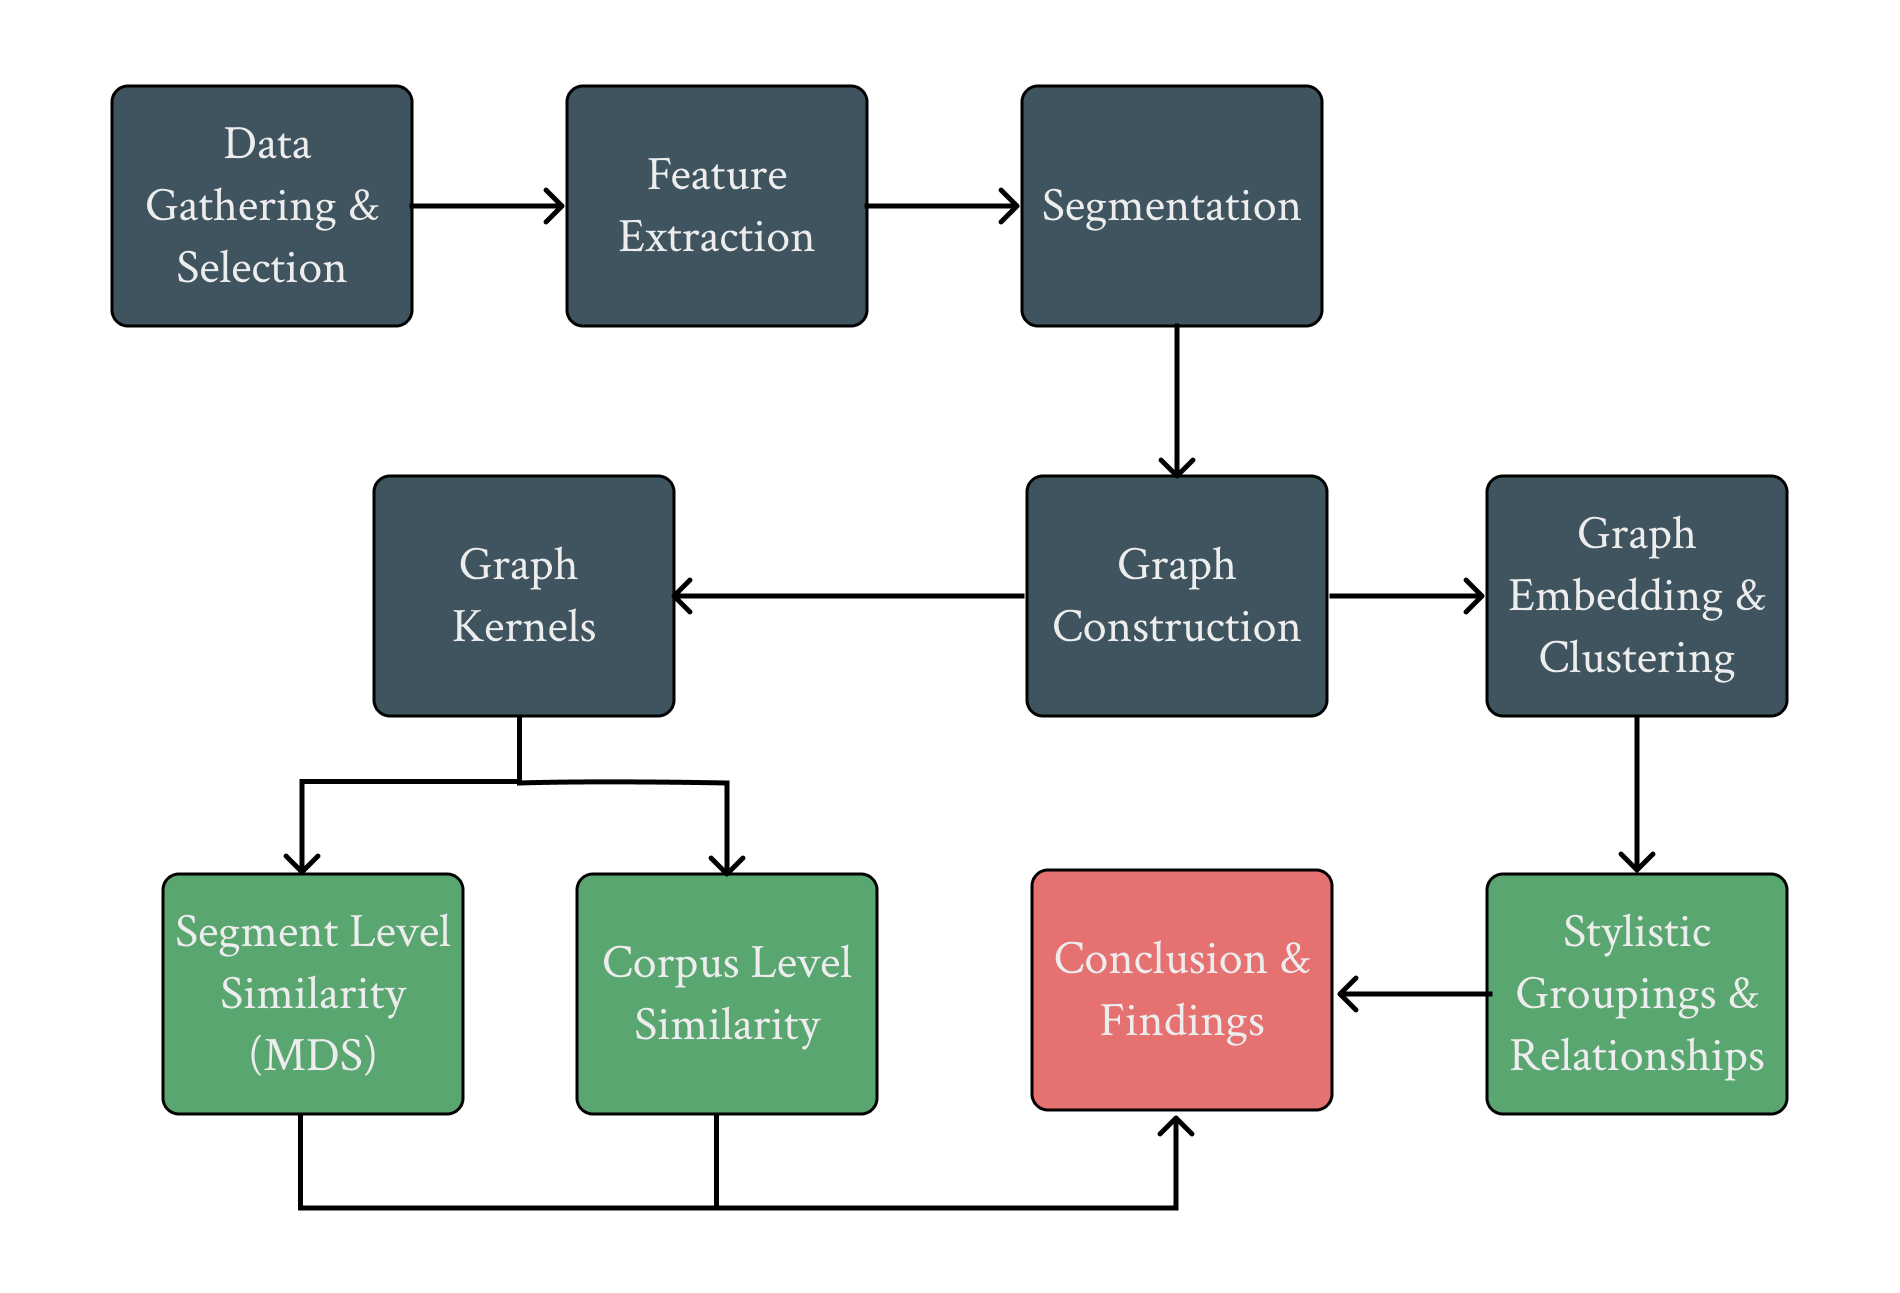
\includegraphics[width=1\linewidth]{Plain_Methodology.png}
Figure 3.1: Methodology Flowchart

This chapter outlines the methodology used in order to construct graph representations of the MusicXML data as a whole. The modification to dynamic time warping will be defined later in the chapter. For consistency of the runtime, the model will be run on a 13th Gen Intel Core i5-13420H processor and an NVIDIA GeForce RTX 4050 laptop GPU.

\section{Preparing for Graph Construction}
The dataset of MusicXML transcriptions of compositions is gathered and then processed using the music21 library. This extracts the symbolic data from the composition and allows it to be represented by a note matrix. This note matrix is then stored in a pandas dataframe \cite{ConananEtAl}.

Afterwards, The notes are labelled with an Implication Realization pattern, following the rules defined by Wen et al \cite{WenEtAl}. The I-R label is added as an additional column in the note matrix \cite{ConananEtAl}.

The note matrix is then segmented into \textit{P} child matrices. Boundaries between segments are defined based on temporal pitch and duration, following the Temporal-Gestalt principles. This will be done using the MIDI Toolbox's segmentation function. Each segment or child matrix will serve as a node in the graph representation.

\section{Graph Construction}
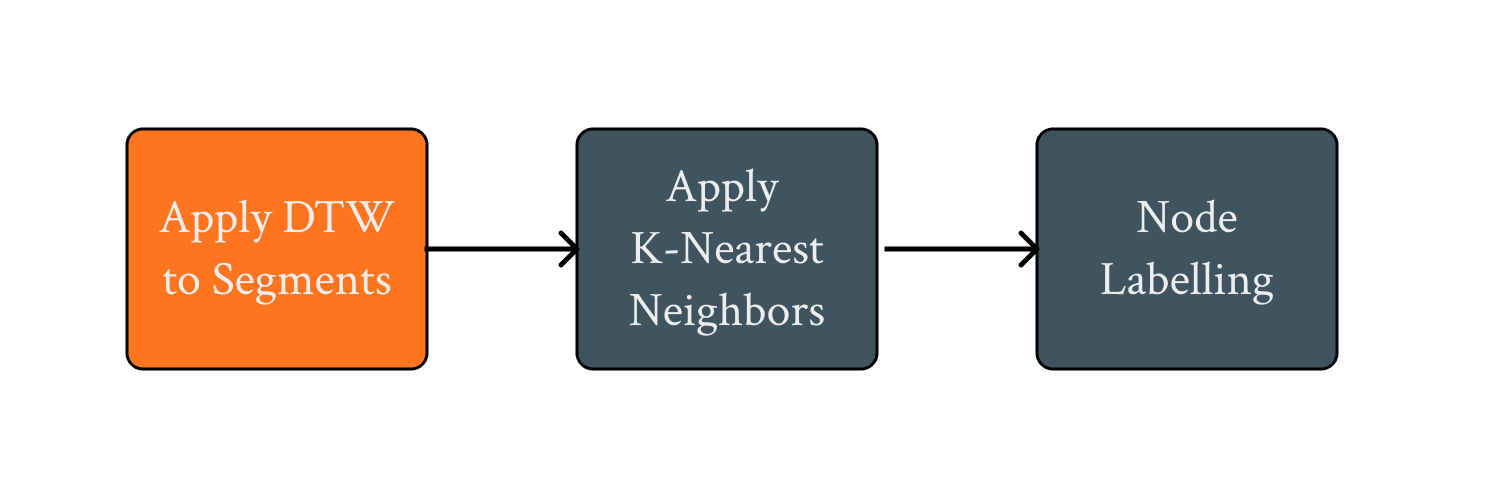
\includegraphics[width=1\linewidth]{Base Graph Construction.png}
Figure 3.2: Graph Construction from Conanan et al.

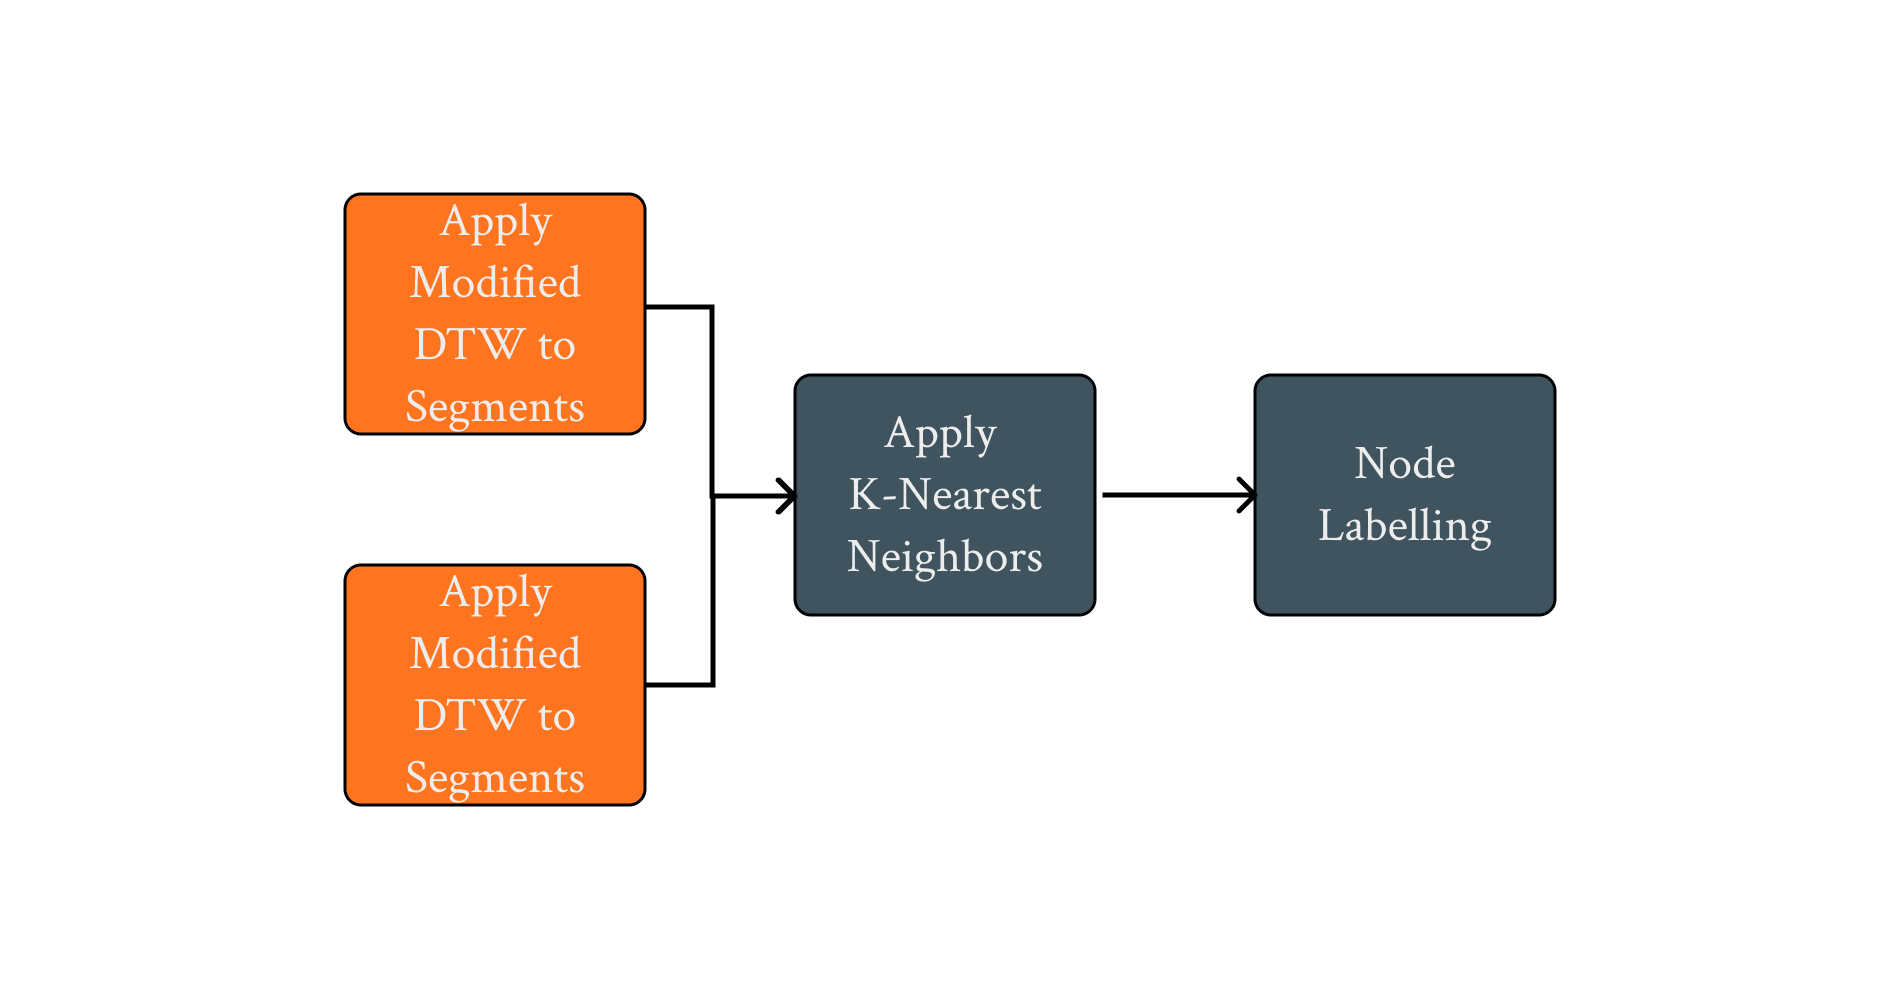
\includegraphics[width=1\linewidth]{Plain NoNormalization Graph Construction.png}
Figure 3.3: Modified Graph Construction

\subsection{Sub-quadratic Dynamic Time Warping}
The DTW-distance computations are performed using an extension of the sub-quadratic $O(n^2 \log\log\log{n}/\log{\log{n}})$ DTW algorithm described in Theorem 2.1 in the Gold and Sharir paper \cite{OmerGold}.The DTW algorithm  from Gold and Sharir is extended to work with two sequences of different lengths, referred to as the $m\le n$ case, as well as to be able to work with points in higher dimensional spaces (in this case, $\mathbb{R}^8$), which Gold and Sharir also covered in section 4.1 of their paper. For higher dimensions, the algorithm functions as described with no significant changes.

The SMAWK algorithm will not be implemented in this paper in order to focus on the base algorithm described by Gold and Sharir in their paper. Nevertheless, $O(n^2 \log\log\log n / \log \log n)$ will still be an improvement to the existing $O(n^2)$ runtime of DTW.

In the actual implementation of the algorithm, it has been divided into six modules for the sake of better modularity and improved tracing of the algorithm. The modules and titles are as follows:
\begin{enumerate}
    \item Segmenting the Input Sequences
    \item Calculating the Boxes
    \item Determining the Paths
    \item Choosing Shortest Paths
    \item Identifying the Optimal Path
    \item Tracing the Complete Path
\end{enumerate}

Before discussing Gold and Sharir's algorithm, we describe below Chan's divide-and-conquer algorithm for the bichromatic dominating pairs problem \cite{ChanDominance}. This algorithm, which we denote $\text{dom}(R,B,d')$ returns all pairs of points in $\mathbb{R}^d$, one point $\vec{r}=(r_1,r_2,\dotsc,r_d)$ from a set $R$ and one point $\vec{b}=(b_1,b_2,\dotsc,b_d)$ from a set $B$, such that for all $i\in\{1,2,\dotsc,d\}, r_i\le b_i$, in $O(c_\epsilon^dn^{1+\epsilon}+K)$ time.

Let $L=R\cup B$, $n=|L|$. Let $d'\le d$. ($d'$ serves as a ``pointer'' to which dimension is being looked at for each recursive call.) There are two base cases.
First, if $n=1$, then no pair of points can be formed, and thus we return $\text{dom}(L,R,d')=\{\}$. Second, if $d'=0$, then we return all pairs of points, i.e., $\text{dom}(L,R,0)=R\times B$.

If $n>1$ and $d'>0$, then we proceed with the recursive case. Let $m$ be the median of the $d'$-th coordinates of all points in $L$. We form the sets
\begin{align*}
    R_{l} = \{\vec{r}=(r_1,r_2,\dotsc,r_d)\mid\vec{r} \in R, r_{d'}\le m\} \\
    R_{r} = \{\vec{r}=(r_1,r_2,\dotsc,r_d)\mid\vec{r} \in R, r_{d'}> m\}   \\
    B_{l} = \{\vec{b}=(b_1,b_2,\dotsc,b_d)\mid\vec{b} \in B, b_{d'}\le m\} \\
    B_{r} = \{\vec{b}=(b_1,b_2,\dotsc,b_d)\mid\vec{b} \in B, b_{d'}> m\}
\end{align*}
We then perform recursive calls on $(R_l,B_l,d')$, $(R_r,B_r,d')$, and $(R_l,B_r,d'-1)$. (Note that for any $\vec{r}\in R_l$ and $\vec{b}\in B_r$, $r_{d'}<b_{d'}$. Thus, our condition is satisfied for dimension $d'$, and so we call dom on $d'-1$.)
To combine the solutions, we return

$\text{dom}(R,B,d')=\text{dom}(R_l,B_l,d')\cup \text{dom}(R_r,B_r,d') \cup \text{dom}(R_l,B_r,d'-1).$


Module 1: Segmenting the Input Sequences contains half of the Stage 0: Preparations from Gold and Sharir's original paper \cite{OmerGold}. The module takes the two input sequences and segments them into subsqeuences that overlap. Afterwards, a distance matrix or \textit{box} is calculated using every pair of subsequences from A and B. The expected input of this module is two sequences and the expected output are distance matrices for every pair of subsequences.

Module 2: Calculating the Boxes contains the latter half of Stage 0: Preparations. Firstly, given the subsequence size used, the module calculates the positions of $L$ and $R$ in the sub-quadratic DTW. Afterwards, it tests every pair of positions between $L$ and $R$ in order to find the \textit{admissible pairs}. The expected input is a box and the expected output are the admissible pairs of positions. The positions of $L$ and $R$ are also stored.

Module 3: Determining the Shortest Paths begins Stage 1: Preprocessing of the sub-quadratic DTW algorithm \cite{OmerGold}. Given the positions of $L$ and $R$ from Module 2, all possible positions of paths are enumerated. Afterwards, sign assignment is performed on the terms to prepare them for Chan's algorithm in Module 4. The expected input of Module 3 are the pairs of positions and the expected output are the possible paths per pair.

Module 4: Choosing the Shortest Paths is an implementation of Chan's Bichromatic Dominance Reporting Algorithm as used by Gold and Sharir \cite{OmerGold}. Using Chan's Algorithm, the shortest path amongst the possible paths is identified and reported per box. The expected input is are the paths and the expected output is a single shortest path chosen.

Module 5: Identifying the Optimal Path is the first half of Stage 2: Compact Dynamic Programming in the sub-quadratic DTW algorithm \cite{OmerGold}. This Module attempts to identify what value of L and R will produce the shortest path amongst all pairs of positions, leading to a single definitive shortest path per box.

Module 6: Tracing the Complete Path is the last stage of the algorithm as the shortest paths from each box are connected using the overlapping subsequences. This leads to a final connected path for the input sequences.

\subsubsection{Sequences of Different Lengths}
Extending the algorithm to work with sequences of unequal lengths will not significantly change the implementation of the algorithm. Let $A$ and $B$ be two sequences of unequal lengths.

In the preparation stage, the sequences will be decomposed into boxes of size $g$, however, the number of boxes from $A$ and $B$ will no longer be equal. Let $A$ be decomposed into $s$ subsequences where $s$ is $\frac{n_A }{g-1}$. $B$ will also be decomposed into $\frac{n_B}{g-1}$ subsequences, but it cannot be the same variable as $A$ since $A$ and $B$ have different lengths. The number of subsequences for $B$ will be denoted as $r$.

The calculation of distance matrices between pairs of subsequences of $A$ and $B$ will still produce boxes of size $g \times g$, however, the number of boxes will no longer be $s^2$ or $s \times s$ but rather $s \times r$. Since the boxes will still be of size $g \times g$, the calculation of staircase paths and shortest paths will still remain the same as described by Gold and Sharir. The preprocessing stage of the algorithm will stay the same since it involves only operations within the boxes.

In the compact dynamic programming stage of the algorithm, the number of horizontal boxes and vertical boxes will not be equal due to the unequal lengths of the sequences $A$ and $B$, however, there will be no change to the logic of the algorithm. Computing minimal pairs for each box will remain the same as described by Gold and Sharir. Finding the minimal cost $M[\ell, m]$ from $(0,0)$ will still have the same logic as it is computed horizontally and vertically, independent of each other.

\subsection{Parallelization}
To speed up the quadratic computation barrier of DTW, hardware-based parallelization will be used. Based on the results in Campos et al, a discrete NVIDIA GPU will be used for implementing parallelization of DTW as it offers the highest throughput of the different hardware types \cite{GPUParallelization}. In this paper, an NVIDIA GeForce RTX 4050 Laptop GPU will be used. The GPUDTW package will be used to run DTW on the GPU and the code will be adapted from GPUDTW's test script test.py.

\subsection{KNN Graph Construction}
K-Nearest Neighbors (KNN) will be applied onto the segments where each segment is connected to its \textit{k} closest neighbors based on the calculated distance matrix. The connected components are first identified. Afterwards, the closest pairs of nodes between disjoint components are identified and connected. This will be repeated until the graph is completely connected.

\subsection{Node Labels}
In order to prepare for analysis using graph kernels, the nodes will be labelled with a binned expectancy score and dominant I-R symbol, following the I-R framework.

\section{Performance Metrics}
\subsection{Graph Analysis}
First, the intra-graph and inter-graph similarity scores will be computed for the value \textit{k} used in KNN. The Kernighan-Lin algorithm will be applied to a graph in order to segment it into two subgraphs. The Weisfeiler-Lehman Kernel will then be applied in order to compute the intra-graph similarity score. Afterwards, the inter-graph similarity will be computed using the Weisfeiler-Lehman Kernel between two graphs. This process will be done for all graphs and pairs of graphs.

In order to determine the optimal value of \textit{k}, the KNN will be applied and intra-graph and inter-graph similarities will be computed for multiple values of \textit{k}. The optimal value of \textit{k} must have a high intra-graph similarity score, meaning that it is consistent with itself and a lower inter-graph similarity score, meaning that it is distinct from other graphs \cite{ConananEtAl}. For each computed intra-graph and inter-graph similarity score, the following tests are applied in order to further compare the two distributions: Shapiro-Wilk test, Independent two-sample t-test, Mann Whitney U test, False Discovery Rate correction. The following are also computed: Cohen's \textit{d} and Area Under the Curve.

The segment-level similarity between two graphs will be determined through Multidimensional Scaling (MDS). This will be done for all pairs of graphs. Silhouette score will be used in order to evaluate the clustering done by MDS.

Lastly, the clustering of all of the graphs will be evaluated. graph2vec is used  to convert each graph into a vector embedding. K-Means clustering is applied to cluster the vector embeddings and Principal Component Analysis is applied in order to reduce the features to two for visualization.

\subsection{Runtime Measurement}
The runtime of the function will be measured using the time module in Python to subtract the time at the start of the function from the time at the end of the function. This will be done for both the base implementation of DTW used by Conanan et al and the modified implementation of DTW. Furthermore, the time for each step in the model will also be recorded in order to produce a breakdown of the total runtime of the model. The performance metrics described by Adefemi for parallel computing will also be applied and calculated \cite{AdefemiParallelization}.
%\chapter{RESULTS AND DISCUSSION}
\section{Preliminary Results}
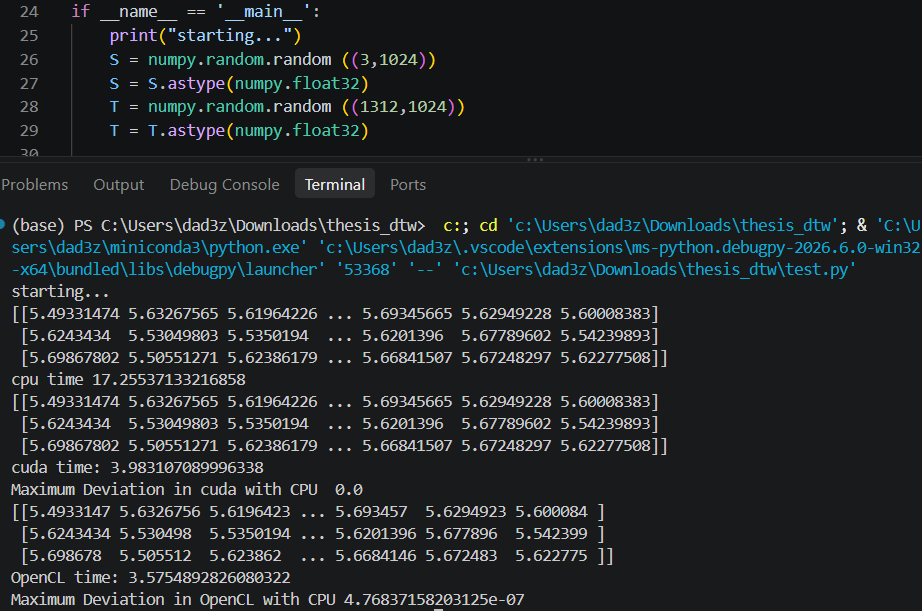
\includegraphics[width=1\linewidth]{prelim1.png}
Figure 4.1: test.py using 3 * 1312

Using a slightly modified version of the provided test.py script from the GPUDTW package, the speed of the CPU to compute DTW can be compared to the speed of the GPU computing DTW using the same inputs. Modifications made include outputing the computed DTW for visual confirmation, removing unnecessary outputs, and lowering the number of data points per sequence due to hardware limitations.

The first array used in testing has 3 sequences with 1024 data points each sequence while the second array has 1312 sequences with 1024 data points each. There are 1024 * 1024 = 1,048,576 cells per pair and 3 * 1312 = 3,936 pairs for a total of 4,127,195,136 cells computed with DTW.

The CPU took an estimated 17.26 seconds while the GPU took an estimated 3.98 seconds through cuda and an estimated 3.58 seconds through OpenCL. Cuda had a 333\% speedup while OpenCl had a 382\% speedup, though cuda no deviation from the CPU's computations while OpenCL's computations match consistently only up to the 6th decimal point. Past the testing stage, only cuda will be used as it is catered towards NVIDIA and to preserve accuracy with results.

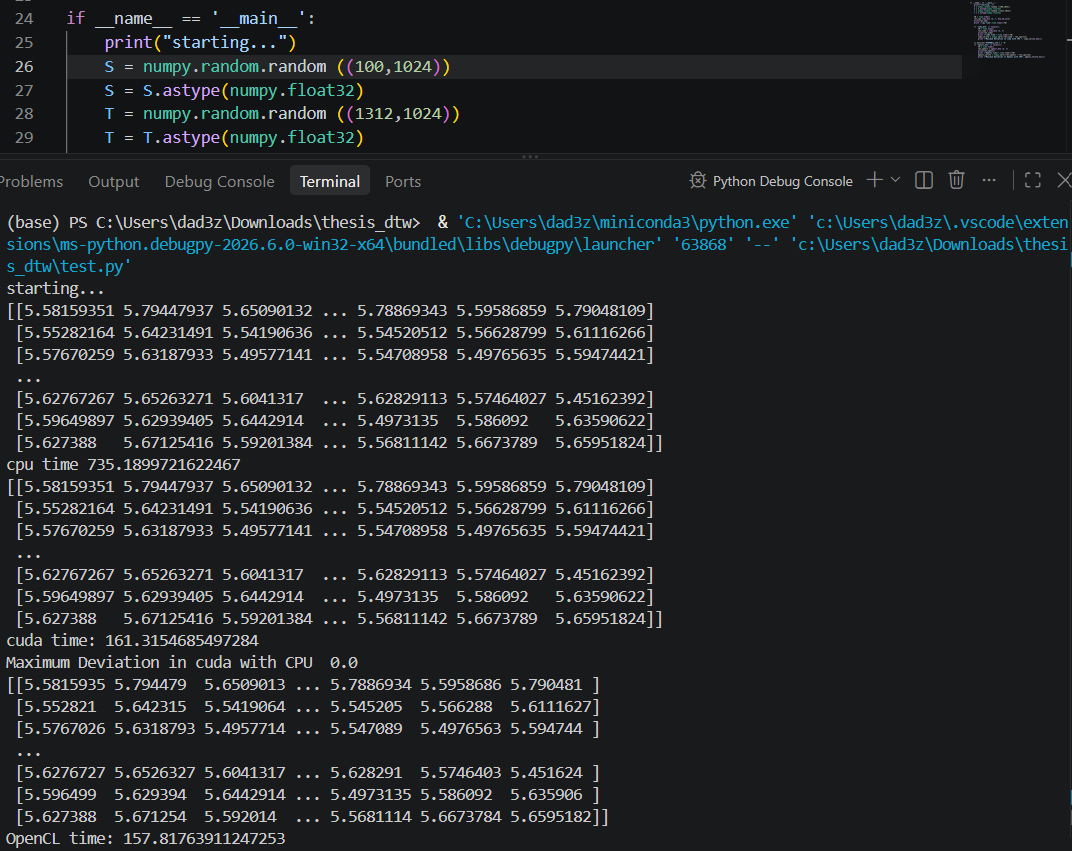
\includegraphics[width=1\linewidth]{prelim2.png}
Figure 4.2: test.py using 100 * 1312

Even with a roughly 33x increase, increasing the amount of cells to be computed to 137,573,171,200 cells, the overall speedup remains relatively consistent with cuda at 355\% speedup and OpenCL at 365\% speedup
%\input{04_results_pub}
%\input{04_results_unpub}
%\input{05_conclusions}
%\input{06_recommendations}
%\input{08_appendices_b_thesisformattingguidelines}

% BIBLIOGRAPHY
\bibliographystyle{abbrv}
\bibliographystyle{plain}
\bibliography{sigproc}
%\input{09_references}
% \BackMatter

%\bibliography{Proposal_Manuscript}
%\addappheadtotoc
%\begin{appendices}
%\chapter{Geolocation Query Visualization}
%\input{08_appendices_a_introductionandsampleguidequestions}
%\chapter{THESIS FORMATTING GUIDELINES}
%\input{08_appendices_b_thesisformattingguidelines}

%\input{08_appendices_method1query}
%\input{08_appendices_method2query}

%\end{appendices}


\end{document}